\documentclass[a4paper,12pt]{article}
\usepackage[utf8]{inputenc}
\usepackage{graphicx}
\usepackage{geometry}
\geometry{left=2.5cm, right=2.5cm, top=3cm, bottom=3cm}
\usepackage{fancyhdr}
\usepackage[portuguese]{babel}
\usepackage{indentfirst}
\usepackage{xcolor}
\usepackage{amsmath}
\usepackage[round, authoryear]{natbib}
\usepackage{subcaption} 
\usepackage{float}      


% cabeçalho
\fancyhf{}
\fancyhead[C]{\small Relatório individual $\bullet$ Sísmica de Refração}
\fancyhead[R]{\thepage}
\renewcommand{\headrulewidth}{0.4pt}
\pagestyle{fancy}

\renewcommand{\figurename}{Figura}


\title{relatorio_parcial_cnpq}
\author{gabriel chagas}
\date{February 2025}



\begin{document}


\begin{center}
    
\includegraphics[width=1.7cm]{usp-logo.png} \hfill 
    
\includegraphics[width=1.6cm]{iagusp-logo.png} 
        
    \vspace{1cm}
    {\Large \textbf{Interpretação de dados reais na Travessa C localizada na Cidade Universitária}}\\[0.5cm]
    {\large \textit{Relatório individual}}\\[1cm]
\end{center}


\textbf{Aluno:} Gabriel Aparecido das Chagas Silva\\

\textbf{Professor(a):} Liliana Alcazar Diogo \\

\textbf{Instituição:} Instituto de Astronomia, Geofísica e Ciências Atmosféricas - IAG USP\\
\headrule{}

\vspace{1cm}



\section{Introdução}

A sísmica de refração é um método de investigação geofísica que estuda o comportamento das ondas refratadas em subsuperfície geradas por uma fonte sísmica, que são registradas por geofones na superfície. Suas aplicações são variadas, amplamente utilizada na engenharia civil, geotecnia e hidrogeologia, por exemplo. A partir dos parâmetros físicos obtidos, é possível inferir e analisar a geologia local e contribuir para as diversas áreas de conhecimento. Nesse relatório, será interpretado dados de sísmica de refração obtidos na Travessa C na Cidade Universitária, na cidade de São Paulo, no ano de 2022 (figura 1). Inicialmente, sabe-se que a região de coleta é movimentada com um fluxo considerável de automóveis e pessoas e a região de coleta era composta por solo, não havendo informação se ele estava seco ou úmido no dia da coleta dos dados. O objetivo é interpretar o comportamento das \textit{wavelets} e estudar a geologia local a partir dos conhecimentos teóricos apresentados em aula e na prática. Por fim, descrever como foi a atividade de campo realizada também na Cidade Universitária, próxima ao ICB (Instituto de Ciências Biomédicas, figura 2). 




\begin{figure}[H]
    \centering
    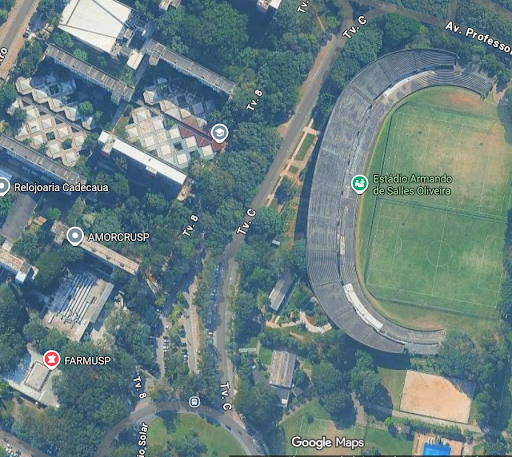
\includegraphics[width=0.5\linewidth]{travessa-c.png}
    \caption{Travessa C, região de coleta dos dados analisados.}
    \label{fig:placeholder}
\end{figure}


\begin{figure}[H]
    \centering
    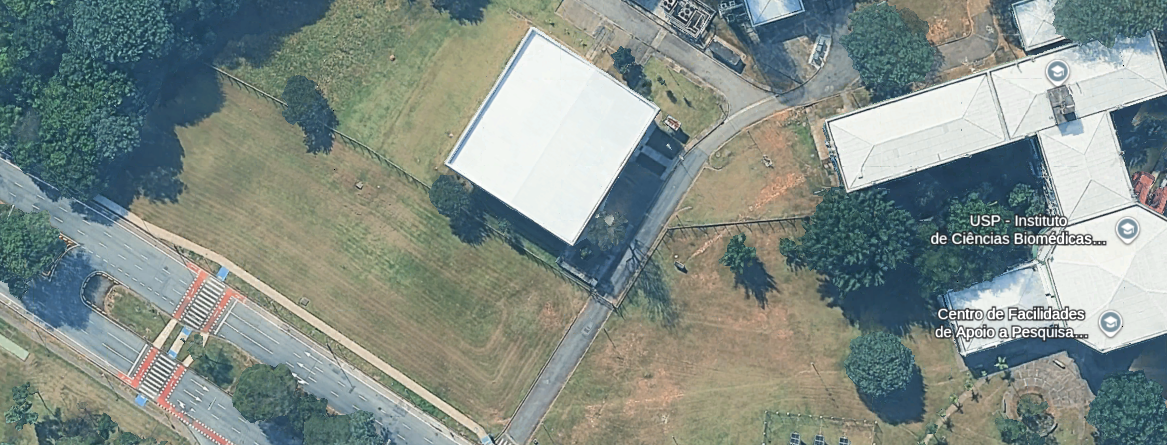
\includegraphics[width=0.5\linewidth]{pratica-2025.png}
    \caption{Região de coleta dos dados em campo, próximo ao ICB.}
    \label{fig:placeholder}
\end{figure}



\section{Contexto Teórico}

\subsection{Interfaces planas}

A fonte sísmica (por exemplo, uma martelada ou explosão de dinamite) gera ondas na subsuperfície. A onda que se propaga diretamente da fonte até o geofone (receptor na superfície) por meio da primeira camada, como o solo, é chamada de \textit{onda direta}. Sua trajetória é a mais curta possível, sendo percebida como uma 'linha reta' em um gráfico. Sua equação está representada em (1):

\begin{equation}
    t(x) = \frac{X}{V_1}
\end{equation}

\noindent
onde $t(x)$ é o tempo em função da distância $x$, $X$ é a distância de offset (posição do geofone em relação ao tiro) e $V_1$ a velocidade no meio.


Pelas primeiras chegadas, percebe-se que em certo ponto a inclinação da reta muda. Esse ponto é chamado de \textit{crossover point}, e indica uma mudança de camada geológica em subsuperfície, um encontro com uma interface que gera uma mudança de velocidade por conta das características físicas do meio. Uma onda refratada em uma interface plana segue a relação representada em (2):

\begin{equation}
    t(x) =  \frac{X}{V_2} + \frac{2h \cos(i_c)}{V_1}
\end{equation}

\noindent
onde $V_2$ é a velocidade da onda na segunda camada, $h$ é a espessura e $i_c$ é o ângulo de incidência crítica dado por um caso particular da \textit{Lei de Snell}, quando a refração é crítica:

\begin{equation}
    \frac{\sin(\theta_1)}{V_1} = \frac{\sin(\theta_2)}{V_2}, \theta_2 = \frac{\pi}{2} \implies \frac{\sin(\theta_1)}{V_1} = \frac{\sin(\frac{\pi}{2})}{V_2}  \implies i_c = \sin^{-1} \frac{V_1}{V_2}
\end{equation}

\noindent
onde $\theta$ é o ângulo de incidência. O segundo termo de (2) é chamado de tempo de intercepto $t_i$; o ponto onde a reta cruza o eixo y do gráfico. Isolando a espessura $h$, obtemos uma equação para esse parâmetro:


\begin{equation}
    h = \frac{V_i t_i}{2 \cos(i_c)}
\end{equation}


Dessa forma, é possível generalizar a equação de uma onda refratada para $n$ camadas planas, dada por:

\begin{equation}
    t_n(x) = \frac{X}{V_n} + \sum_{k=1}^{n-1} \frac{2h_k \cos(i_k)}{V_k}
\end{equation}

\noindent
que mostra que o tempo de intercepto é a soma do atraso de todos atrasos causados pelas camadas acimas da atual. 

\subsection{Interfaces inclinadas ou irregulares}

As interfaces geológicas podem não ser planas, ou podem ser planas mas inclinadas com ângulo $\gamma$ em relação a superfície, que chamamos de \textit{mergulho}. 

Quando uma camada mergulha, a velocidade observada na superfície não é a velocidade real da onda, mas sim uma \textit{velocidade aparente}. Ela parece mais rápida quando a fonte está  acima da parte mais profunda da camada, com um tiro do sentido \textit{downdip} para o \textit{updip}; e parece mais devagar quando a fonte está acima de uma parte mais rasa da camada, com um tiro do sentido \textit{updip} para o \textit{downdip}. Essa relação é observada nas equações abaixo, de forma generalizada.

\begin{equation}
    \frac{1}{V_{ap_{down_{i}}}} = \frac{\sin(i_{c_{i}} + \gamma_i)}{V_i}, \quad \frac{1}{V_{ap_{up_{i}}}} = \frac{\sin(i_{c_{i}} - \gamma_i)}{V_i}
\end{equation}

Com a equação (6), é possível inferir a velocidade real das camadas a partir das velocidas aparentes obtidas no gráfico de \textit{plot}, quando é feito dois tiros, que chamamos de tiro direto (próximo ao que definimos como origem da nossa geometria e arranjo de geofones) e tiro reverso (próximo ao ponto mais longínquo do sistema). A partir das velocidades reais, é possível calcular a espessura abaixo dos pontos de tiro com  a equação (4). Dessa forma, pode-se conectar com uma linha reta as duas espessuras calculadas e estimar a geometria da camada inclinada. Esse método se chamada \textbf{Interceptação no Tempo}. 


Para o caso de uma interface não-plana e irregular, a aproximação com o método de interceptação no tempo pode não ser válida. Para estimar essa geometria, o método chamado de \textbf{Recíproco} calcula a profundidade ponto a ponto, abaixo de cada geofone, sendo mais robusto e confiável. Para isso, usa-se o conceito de \textit{tempo de atraso}: a diferença entre o tempo real de percurso da onda refratada e o tempo que a onda teria levado para viajar a mesma distância horizontal se ela estivesse se movendo inteiramente na velocidade real do refrator. A equação do tempo de atraso (plus-minus) é dada por:

\begin{equation}
    a_X = \frac{1}{2} (t_{AX} + t_{BX} - t_{AB}) 
\end{equation}

\noindent
onde $a_x$ é o tempo de atraso, $t_{AX}$ o tempo de viagem da onda no tiro direto, $t_{BX}$ idem mas para o tiro reverso, e $t_{AB}$ o tempo recíproco (duração da propagação no refrator). Dessa forma, podemos calcular a espessura $h$ abaixo do i-ésimo geofone, por meio de:

\begin{equation}
    h_x = a_x \frac{V1}{\cos(i_c)}
\end{equation}

Com (8), pode-se calcular a profundidade abaixo de cada geofone e fazer um modelo estimado da geometria da interface, a partir do método recíproco. 


\section{Ferramentas e materiais utilizados}

\subsection{Equipamentos de campo}

Para o campo, tanto o da prática de 2025 quanto o da coleta de dados de 2022, foram utilizados 96 geofones ligados entre si e à um sismógrafo conectado a um PC blindado próprio para a atividade de campo. Como fonte sísmica, foi utilizado uma marreta com um \textit{trigger}, que registra o tempo zero a partir do impacto do tiro com a superfície, gerando as ondas sísmicas. 

\subsection{Processamento e Interpretação}

Para o pré-processamento e a marcação dos picks de primeira quebra, foram exploradas duas abordagens principais. A ferramenta padrão utilizada foi o \textit{Seismic Unix (SU)}, software nativo do sistema operacional Linux, que permitiu a visualização inicial dos sismogramas e a aplicação de filtros para a melhoria do sinal. Em paralelo, foi desenvolvida uma solução alternativa utilizando a linguagem de programação \textit{Python}, com o auxílio das bibliotecas \textit{ObsPy} e \textit{matplotlib}. Esta abordagem se mostrou muito promissora, possibilitando a criação de uma ferramenta de picking interativa e a implementação de filtros de frequência, replicando as principais funcionalidades do Seismic Unix. Embora o SU tenha sido a base para a metodologia, a exploração com Python demonstrou grande potencial para trabalhos futuros.

Quanto ao plot das retas geradas pelos picks e os ajustes de reta com o Método dos Mínimos Quadrados (MMQ), foi utilizado a linguagem de programação \textit{Python} em um ambiente do \textit{Jupyter Notebook}, que permitiu a manipulação e interpretação dos picks e suas retas por meio do \textit{matplotlib} e o \textit{numpy}, bibliotecas da linguagem. 


\section{Procedimento de coleta de dados}

Para as atividades de campo, tanto na prática de 2025 quanto na coleta de dados de 2022, os procedimentos de aquisição foram semelhantes. Foi utilizado um arranjo sísmico com 96 geofones verticais, dispostos com um espaçamento constante de $dx=1m$ entre si. Durante a montagem da linha, buscou-se a maior linearidade possível entre os sensores, garantindo que estivessem firmemente acoplados ao solo para otimizar a recepção do sinal.

A geometria de aquisição incluiu tiros diretos e reversos, realizados tanto de forma interna (dentro do arranjo de geofones) quanto externa (fora das extremidades do arranjo), com o objetivo de obter uma gama maior de informações e melhorar a cobertura do refrator. Para cada ponto de tiro, era buscado o momento com a menor interferência de ruídos ambientes, como vibrações de automóveis ou pedestres. Após cada disparo com a marreta, a resposta do sinal era observada em tempo real no sismógrafo, permitindo uma avaliação imediata do sinal obtido.

A figura 3 mostra o conteúdo do arquivo txt com a geometria da aquisição dos dados da Travessa C.

\begin{figure}[H]
    \centering
    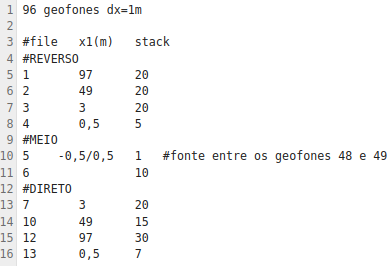
\includegraphics[width=0.5\linewidth]{geometria-aquisicao.png}
    \caption{Geometria de aquisição fornecida pela equipe que realizou a coleta dos dados em campo.}
    \label{fig:placeholder}
\end{figure}




\section{Resultados preliminares}


O resultado direto da aquisição em campo é o sismograma de tiro comum, que é a representação visual da resposta do terreno ao pulso de energia gerado. Neste gráfico, cada linha vertical corresponde a um traço sísmico registrado por um geofone, exibindo as diversas ondas (wavelets) que chegam em função do tempo.

Este dado bruto, no entanto, frequentemente contém ruídos de diferentes fontes que podem mascarar os sinais de interesse, principalmente as primeiras chegadas. Para melhorar a qualidade do dado e facilitar a etapa de marcação dos picks, pode-se refinar os dados com a aplicação de filtros e algumas funções, como:

\begin{itemize}
    \item \textbf{Controle de Ganho:} Aplicado para equalizar as amplitudes ao longo do traço, realçando as chegadas mais tardias que são naturalmente mais fracas.

    \item \textbf{Filtro Passa-Banda (Trapezoidal):} Utilizado para atenuar frequências indesejadas. É eficaz para remover ruídos de baixa frequência, como o \textit{ground roll}, e ruídos de alta frequência, isolando a faixa de frequências do sinal sísmico de interesse.

    \item \textbf{Filtro F-K:} Um filtro que atua no domínio da frequência-número de onda (a partir de uma transformada). Ele é eficiente para remover ruídos coerentes que possuem um mergulho (velocidade aparente) específico, sendo muito eficiente contra o \textit{ground roll} (ondas de superfície com baixa velocidade (baixo valor de k) e alta amplitude).
\end{itemize}


A figura 4 mostra um exemplo de visualização das wavelets em um gráfico, plotado usando o SU, que se mostra ruidoso, mesmo com filtros. No caso dessa imagem, ela é correspondente ao tiro de $n=6$, de acordo com a coluna 'file' do conteúdo mostrado na figura 3, com a geometria de aquisição. A partir daqui, a notação utilizada para referenciar o tiro será essa: o tiro 1 será o tiro correspondente ao índice $n=1$ na coluna 'file' do arquivo de geometria de aquisição. 


\begin{figure}[h]
    \centering
    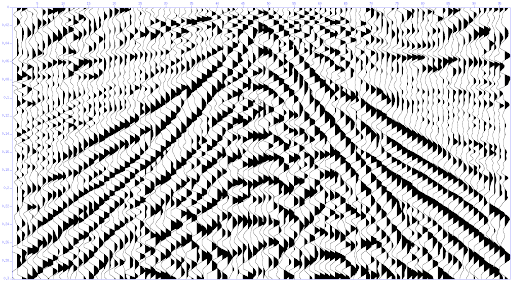
\includegraphics[width=0.5\linewidth]{perfil-n6.png}
    \caption{Gráfico de wavelets do tiro 6, plotado utilizando o Seismic Unix.}
    \label{fig:placeholder}
\end{figure}

A figura 5 mostra o mesmo conjunto de dados de $n=6$ plotado no python, também com filtros aplicados (apesar disso, no momento de realização desse relatório não foi possivel verificar os parâmetros utilizados no plot do SU para aplicar no python). 

\begin{figure}[h]
    \centering
    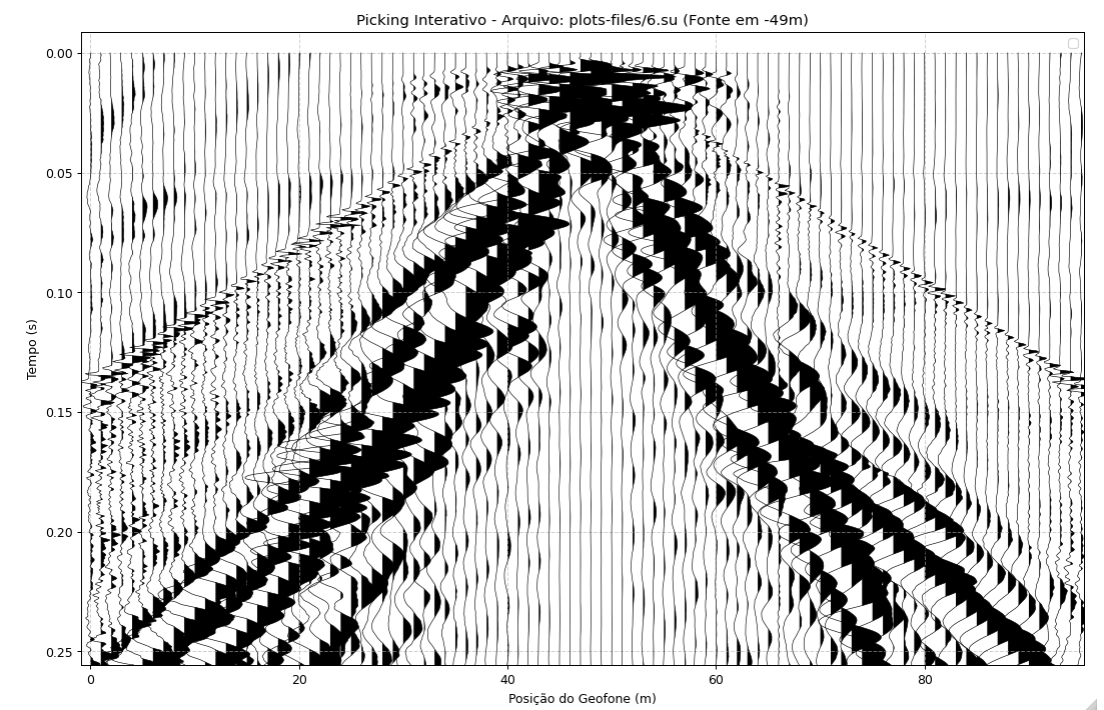
\includegraphics[width=0.5\linewidth]{perfil-n6-python.png}
    \caption{Gráfico de wavelets do tiro 6, plotado utilizando o Python.}
    \label{fig:placeholder}
\end{figure}

Esses são exemplos da visualização obtida para, a partir delas, fazer o processo de picking. A manipulação com filtros e ganho é crucial para fazer os picks adequados que vão permitir a análise e interpretação geológica desses resultados. 

\section{Análise}

A partir dos picks feitos para todos os tiros e ao fazer seus plots no Python, obtém-se o seguinte gráfico da figura 6, que mostra a disposição dos picks (círculos) com base no seu tempo e posição. Como alguns tiros são externos, a onda direta pode não ser visível, pois eles são realizados justamenta para análise da onda refratada como primeira chegada. 

\begin{figure}[h]
    \centering
    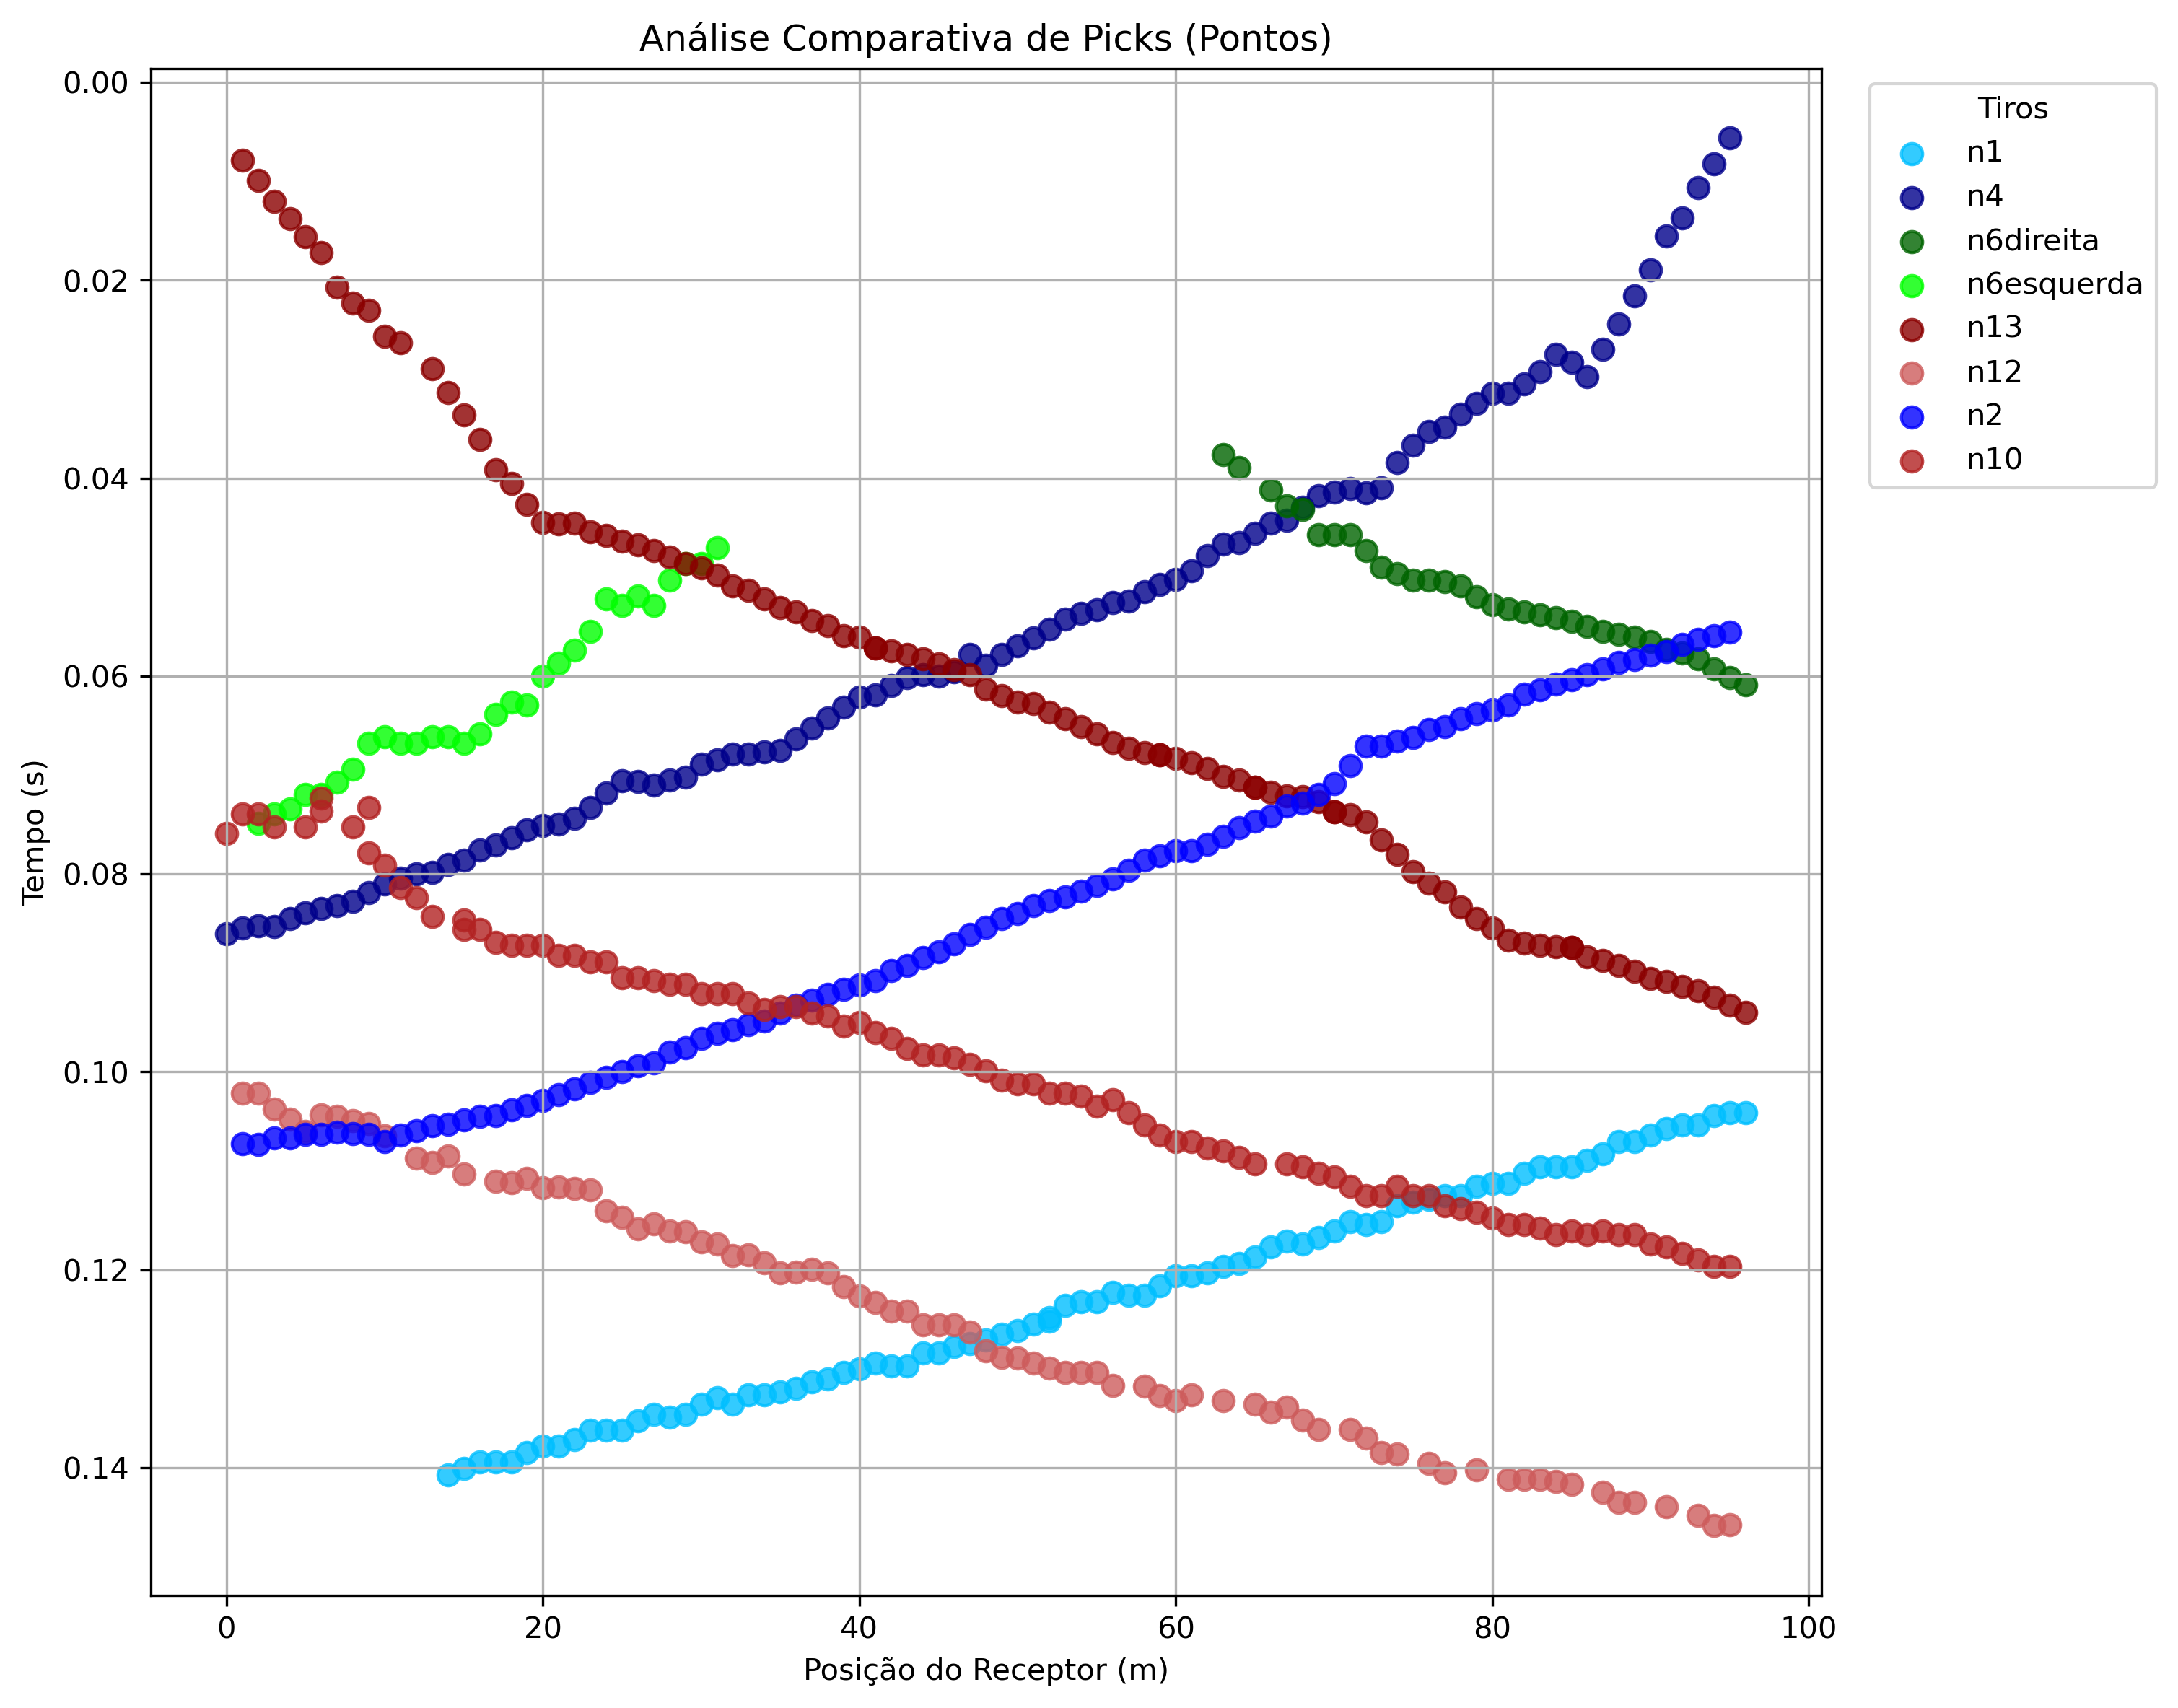
\includegraphics[width=0.5\linewidth]{analise_comparativa_picks.png}
    \caption{Picks em relação à seus parâmetros correspondentes.}
    \label{fig:placeholder}
\end{figure}

Observando esse gráfico, é possível notar que em $n=4$ e $n=13$ a diferença de inclinação entre suas respectivas ondas diretas e refratadas. Para $n=6_{direita}$ e $n=6_{esquerda}$, que são tiros internos centralizados (os mesmos, por exemplo, das figuras 4 e 5) não é possível distinguir as ondas diretas e refratadas, por conta da qualidade ruim dos dados obtidos, mesmo com os filtros aplicados. Ainda com a análise dos pontos, pode-se dizer que há um pararelismo entre os tiros externos o que indica uma mesma velocidade (nesse gráfico de tempo x distância, a velocidade é dada pelo inverso do coeficiente angular), mesmo que em alguns pontos há descontinuidades que podem ser ou ruídos ou uma possível segunda interface (terceira camada). A figura 7 mostra um ajuste de retas com MMQ, separando as ondas diretas visíveis das refratadas correspondentes, e inicialmente sem fazer um corte de regiões distoantes (como, por exemplo, a curvatura em $n=13$ próximo à $x=75m$).

\begin{figure}[h]
    \centering
    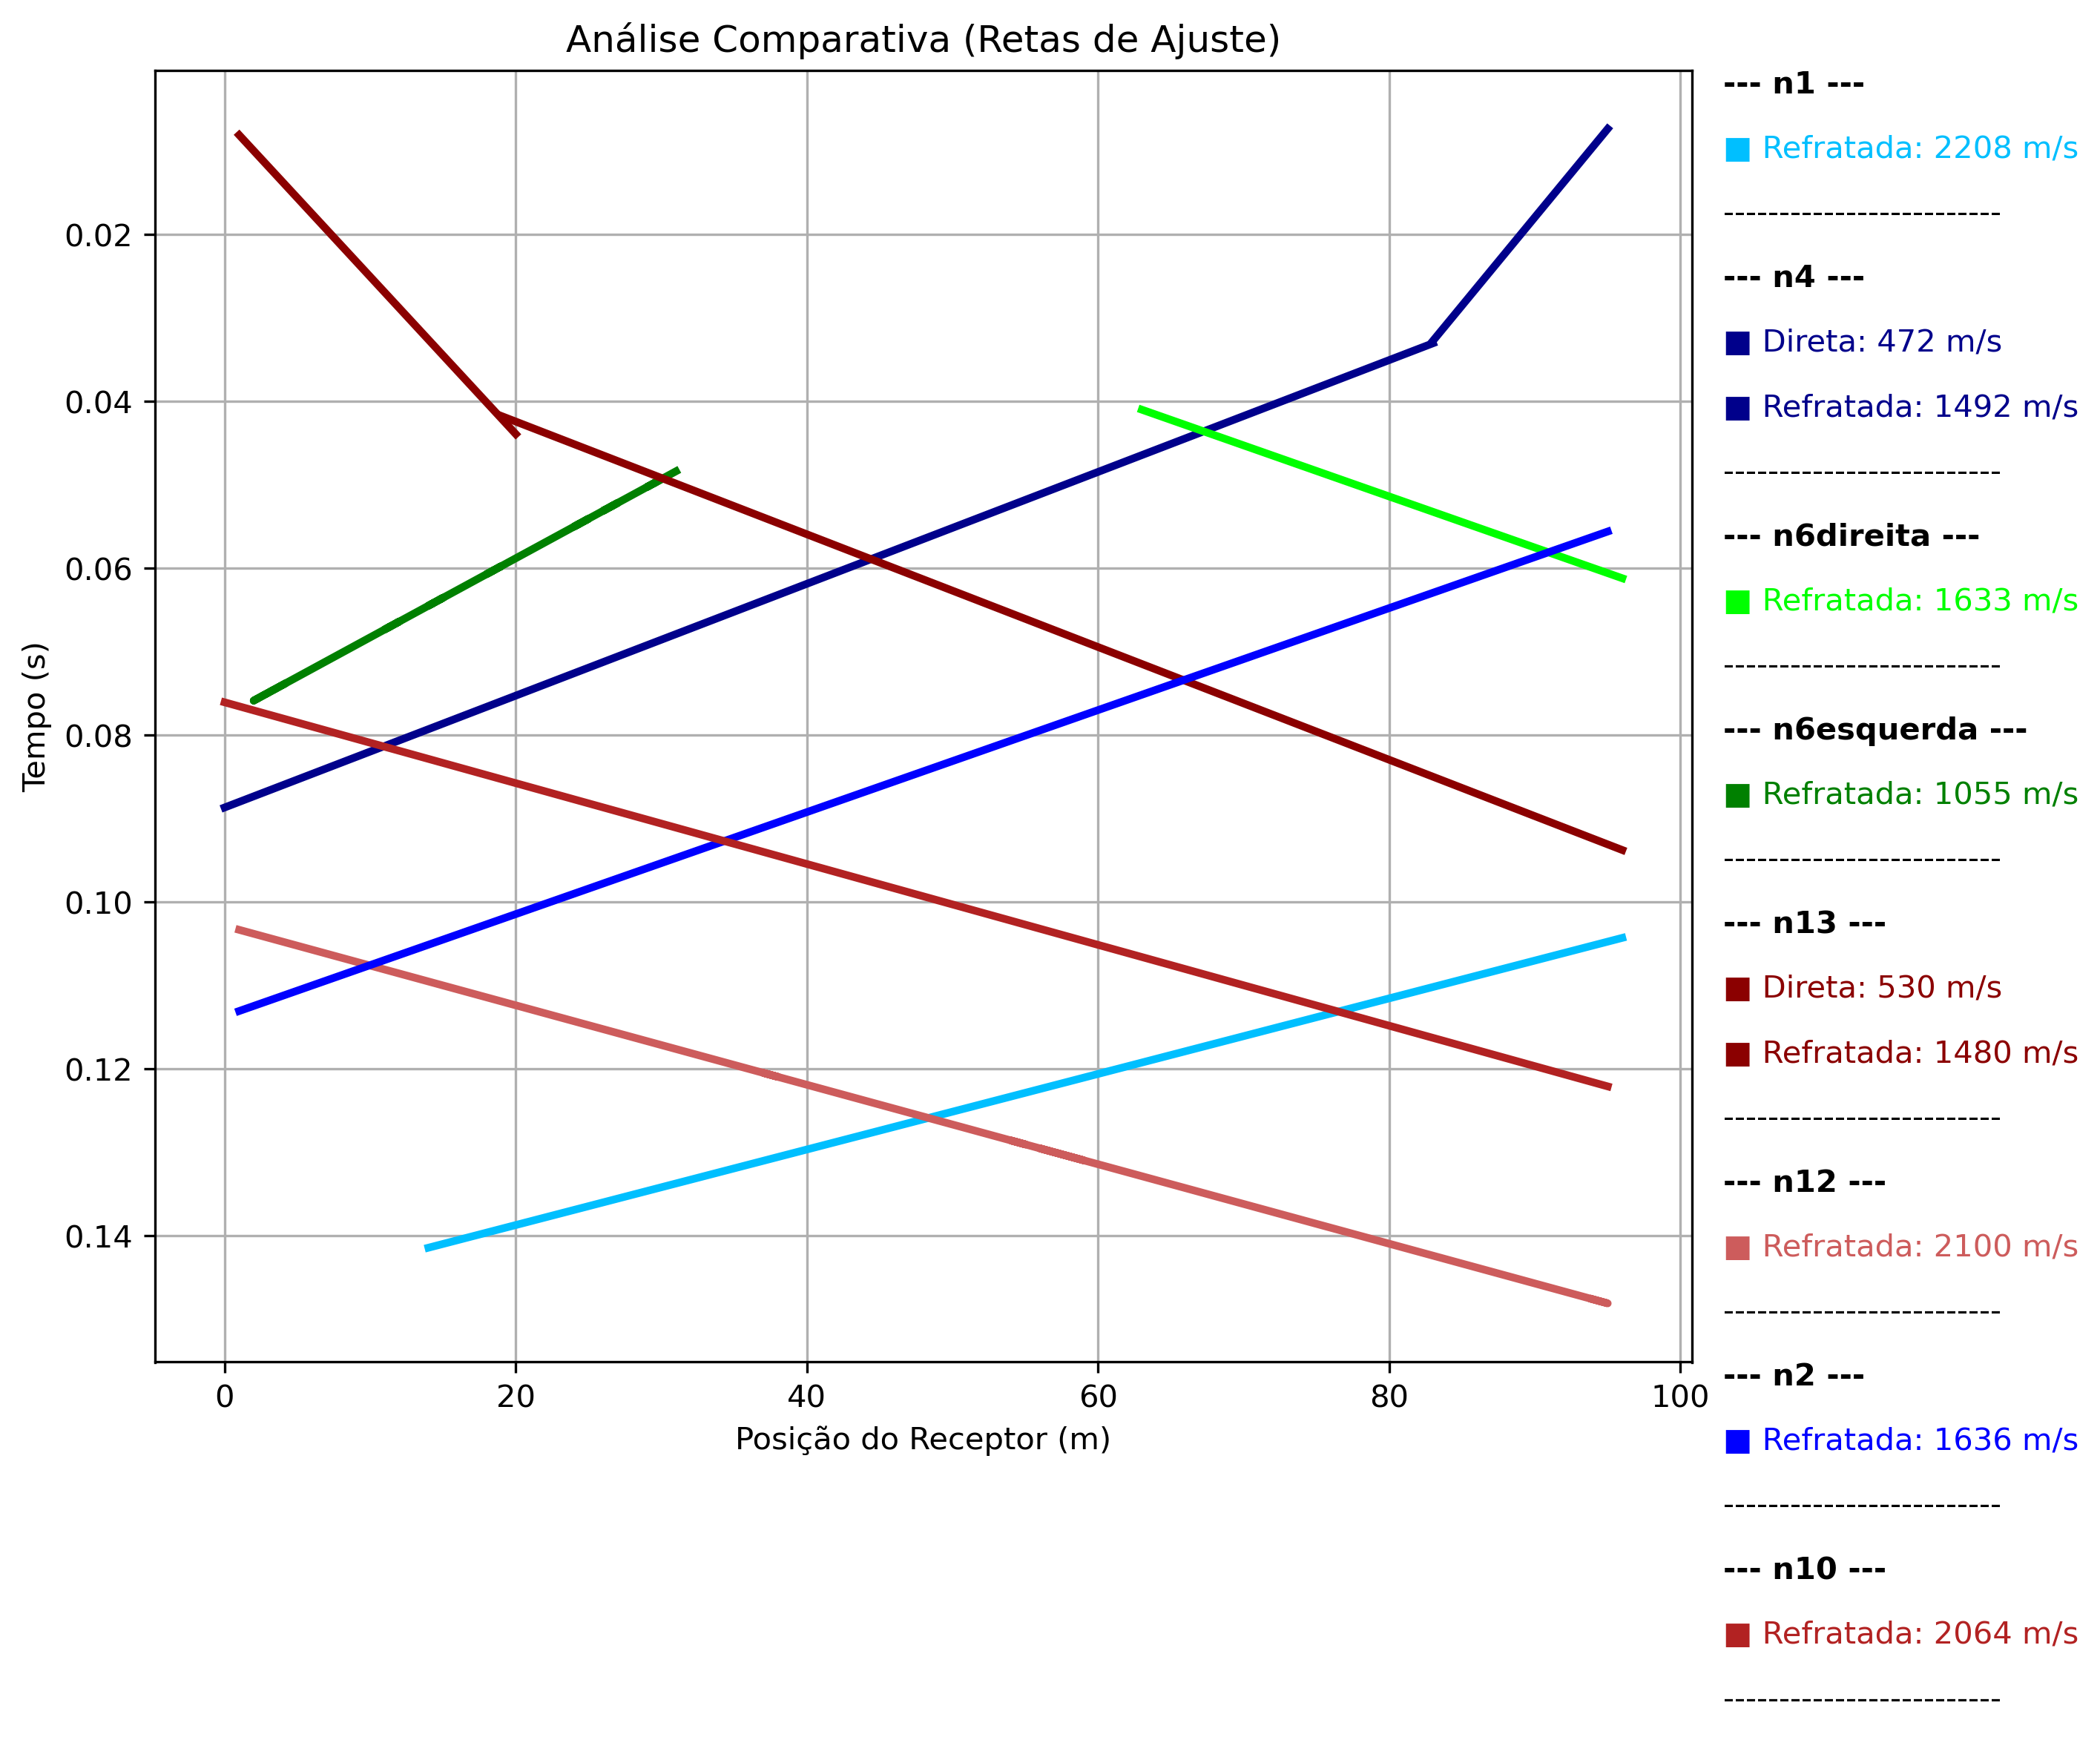
\includegraphics[width=0.5\linewidth]{analise_retas_ajustadas.png}
    \caption{Retas ajustadas sem recortes de possíveis ruídos ou outra interface, e com recorte de ondas diretas e refratadas.}
    \label{fig:placeholder}
\end{figure}

Mesmo sem o recorte de possíveis artefatos, as ondas refratadas se mostram aproimadamente paralelas, como pode-se enxergar em $n=12$ e $n=10$ com velocidades de $2100 m/s$ e $2064 m/s$. Esse paralelismo indica uma mesma velocidade, logo, não houve mudança de camada. A curvatura na parte final de $n=13$ 'puxou' o ajuste para baixo (resultando em uma velocidade de $1480 m/s$, que ali pode ser uma camada diferente ou um efeito de ruído. A figura 8 mostra o mesmo plot da retas agora desconsiderando pontos que podem ser considerados como ruídos.


\begin{figure}[h]
    \centering
    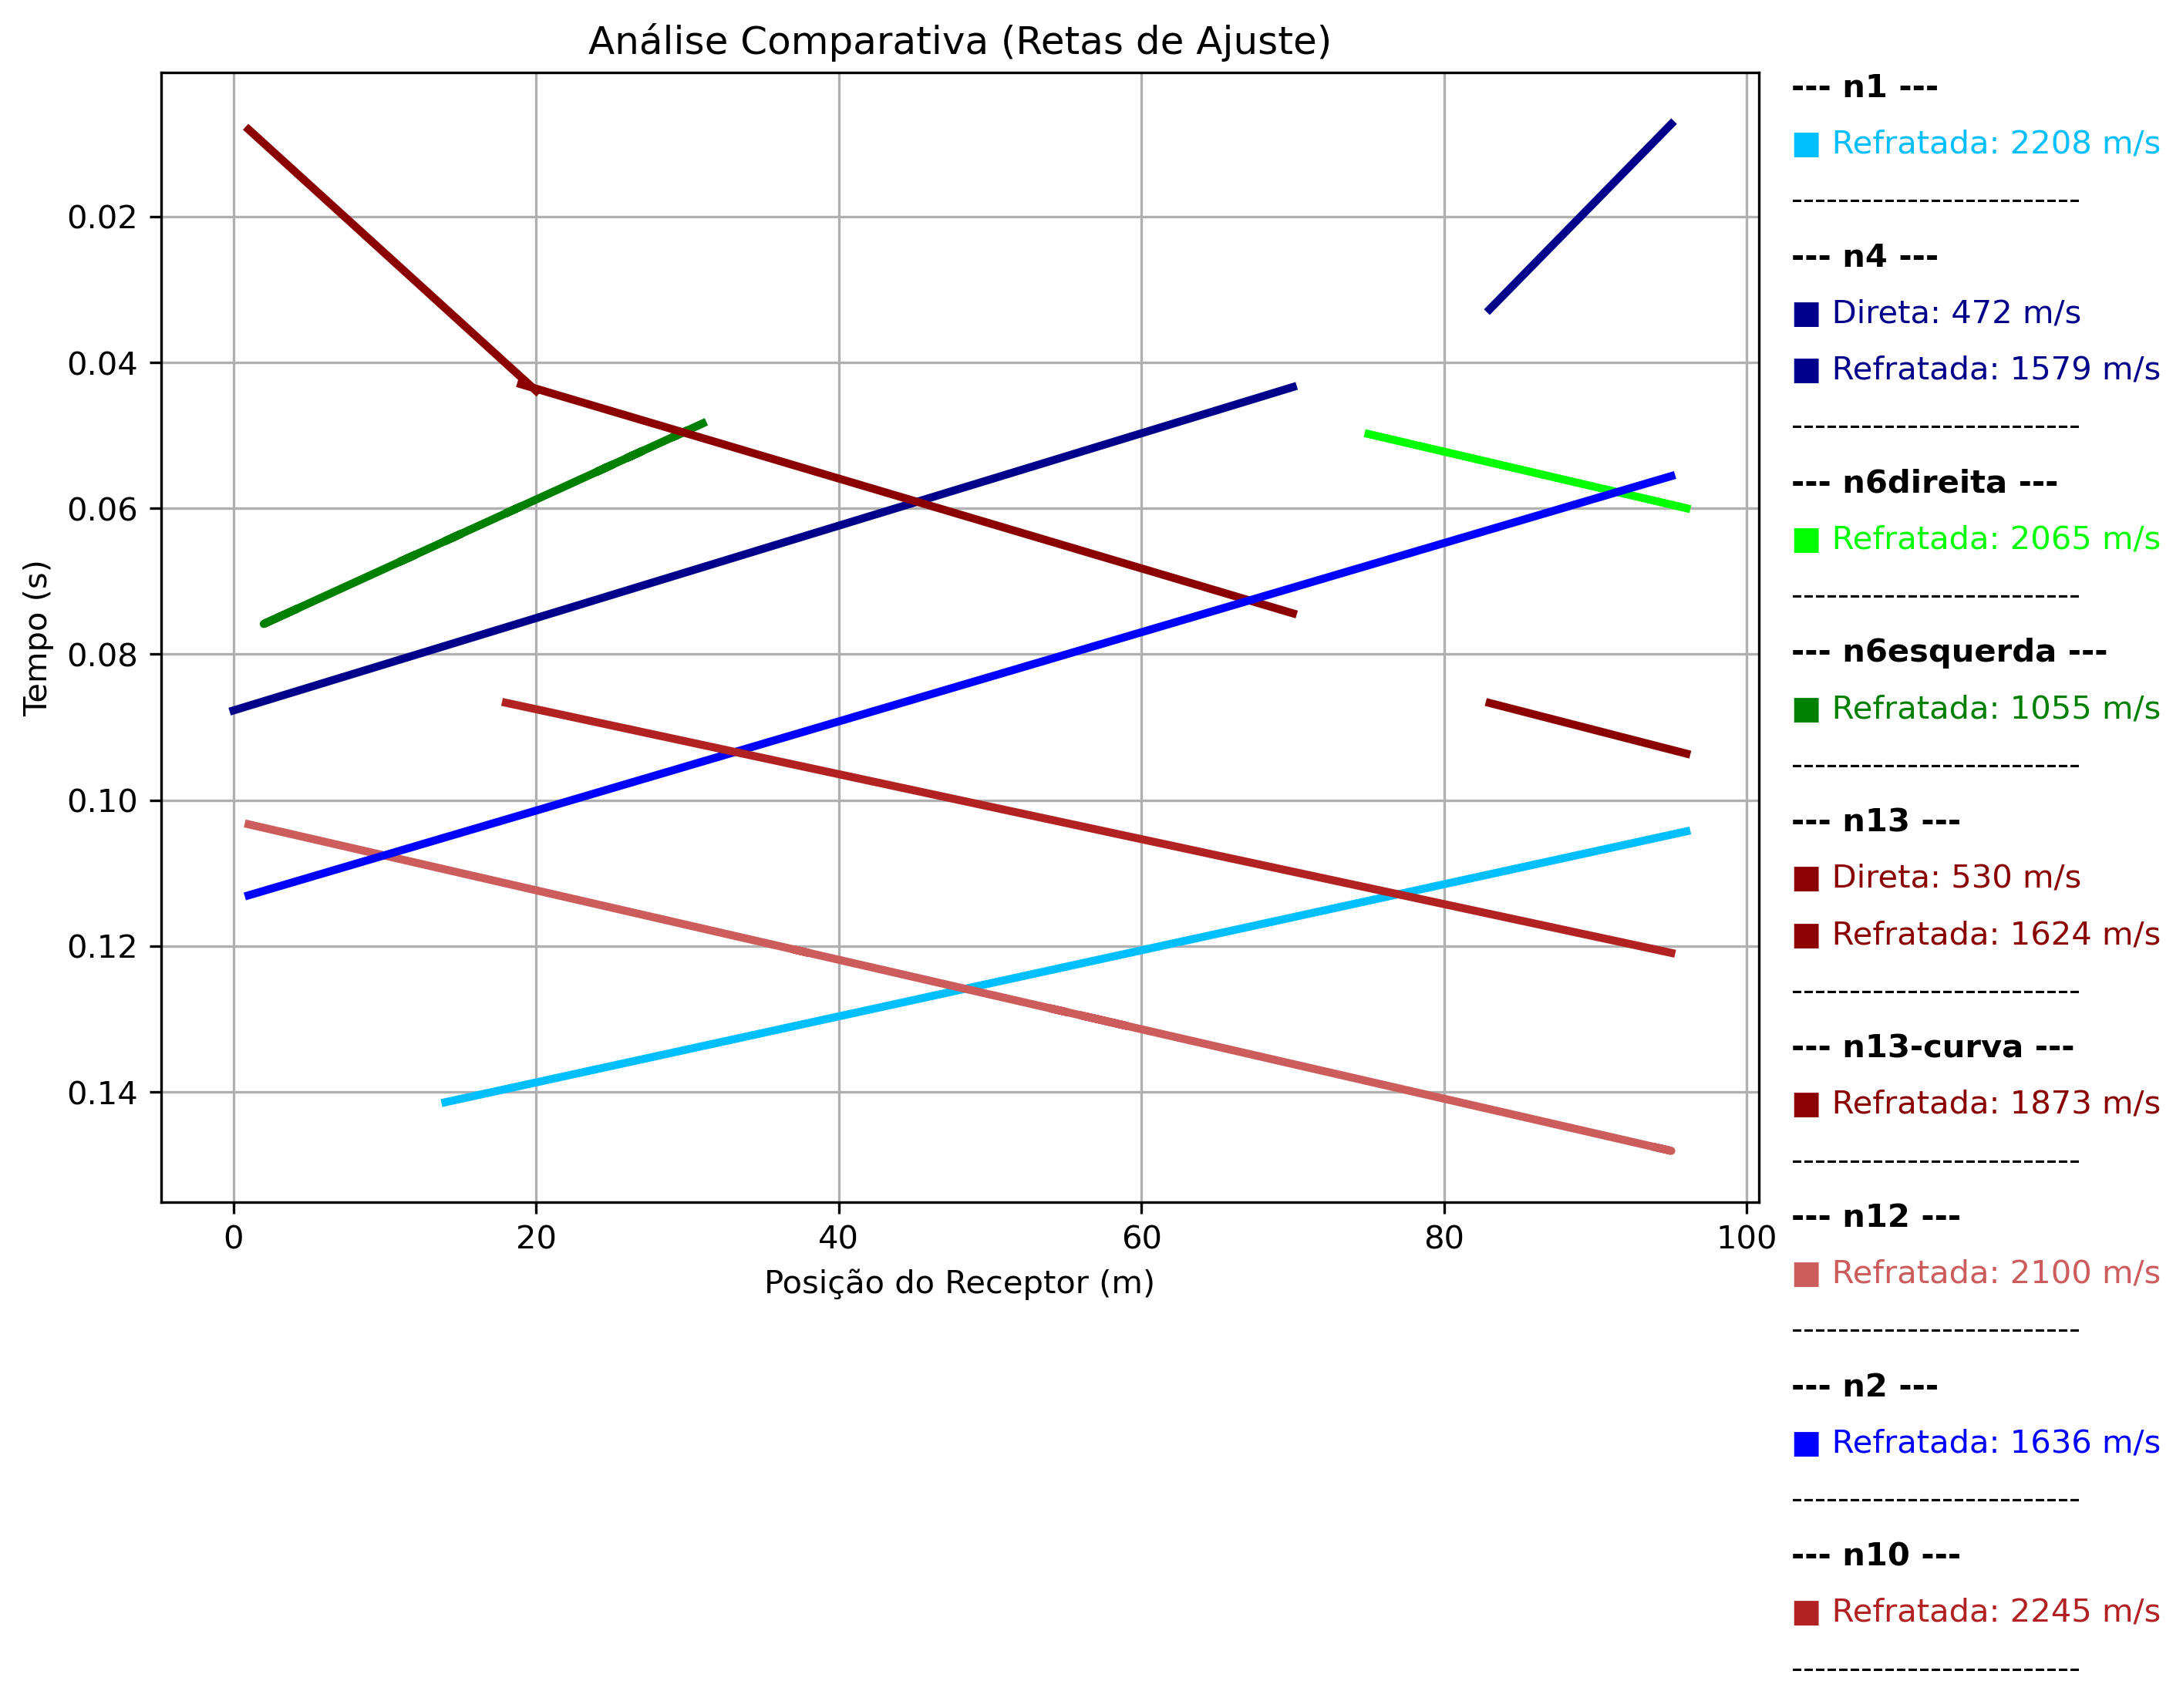
\includegraphics[width=0.5\linewidth]{analise_retas_ajustadas-recorte.png}
    \caption{Ajustes de retas com recorte de regiões possivelmente ruidosas.}
    \label{fig:placeholder}
\end{figure}


Com esse recorte, $n=12$ e $n=10$ ainda continuam aproximadamente paralelas. Agora, com o recorte da refratada $n=13$ em duas partes, sua parte mais próxima a origem assume um valor de velocidade de $1624 m/s$, ainda longe das outras duas retas que, em teoria, ela devia ser paralela. Ainda na análise de $n=13$, a parte linear após a curva observada nos picks (no gráfico, $n=13_{curva}$ apresenta uma velocidadade de $1873 m/s$, mais próxima das outras retas as quais devia ser paralelo. 

Quanto à $n=4$ e $n=2$, seus valores de velocidade se mostram ainda próximos e paralelos, podendo afirmar que eles de fato representam a mesma camada. No entanto, em teoria, era esperado que $n1$ se mostrasse paralelo à esses dois tiros, mas sua velocidade de $2208 m/s$ difere da ordem de grandeza observada nos tiros 4 e 5, de aproximadamente $1600 m/s$. Isso pode indicar um erro de picks, influência de ruído ou uma segunda interface que tem sua primeira chegada observada apenas nas condições de observação do tiro 1. No entanto, a análise geral dos ajustes não parece apontar para a existência de uma segunda interface, mas ela ainda assim não pode ser descartada, devido à quantidade de ruído presente nos dados. 

Para estimar a geometria da malha, será utilizado os métodos de Interceptação no tempo e Recíproco. Para o modelo de ondas escolhidos, será usado os recortes feitos na figura 8, com $n=13$ e $n=4$ que possuem clara distinção entre suas ondas diretas e refratadas. Para a velocidade da refratda do tiro 13, será utilizada a calculada por $n=13_{curva}$, presente no gráfico da figura 8. A figura 9 mostra o análise combinada dessas duas ondas, com seus recortes devidamente feitos. 

\begin{figure}[H]
    \centering
    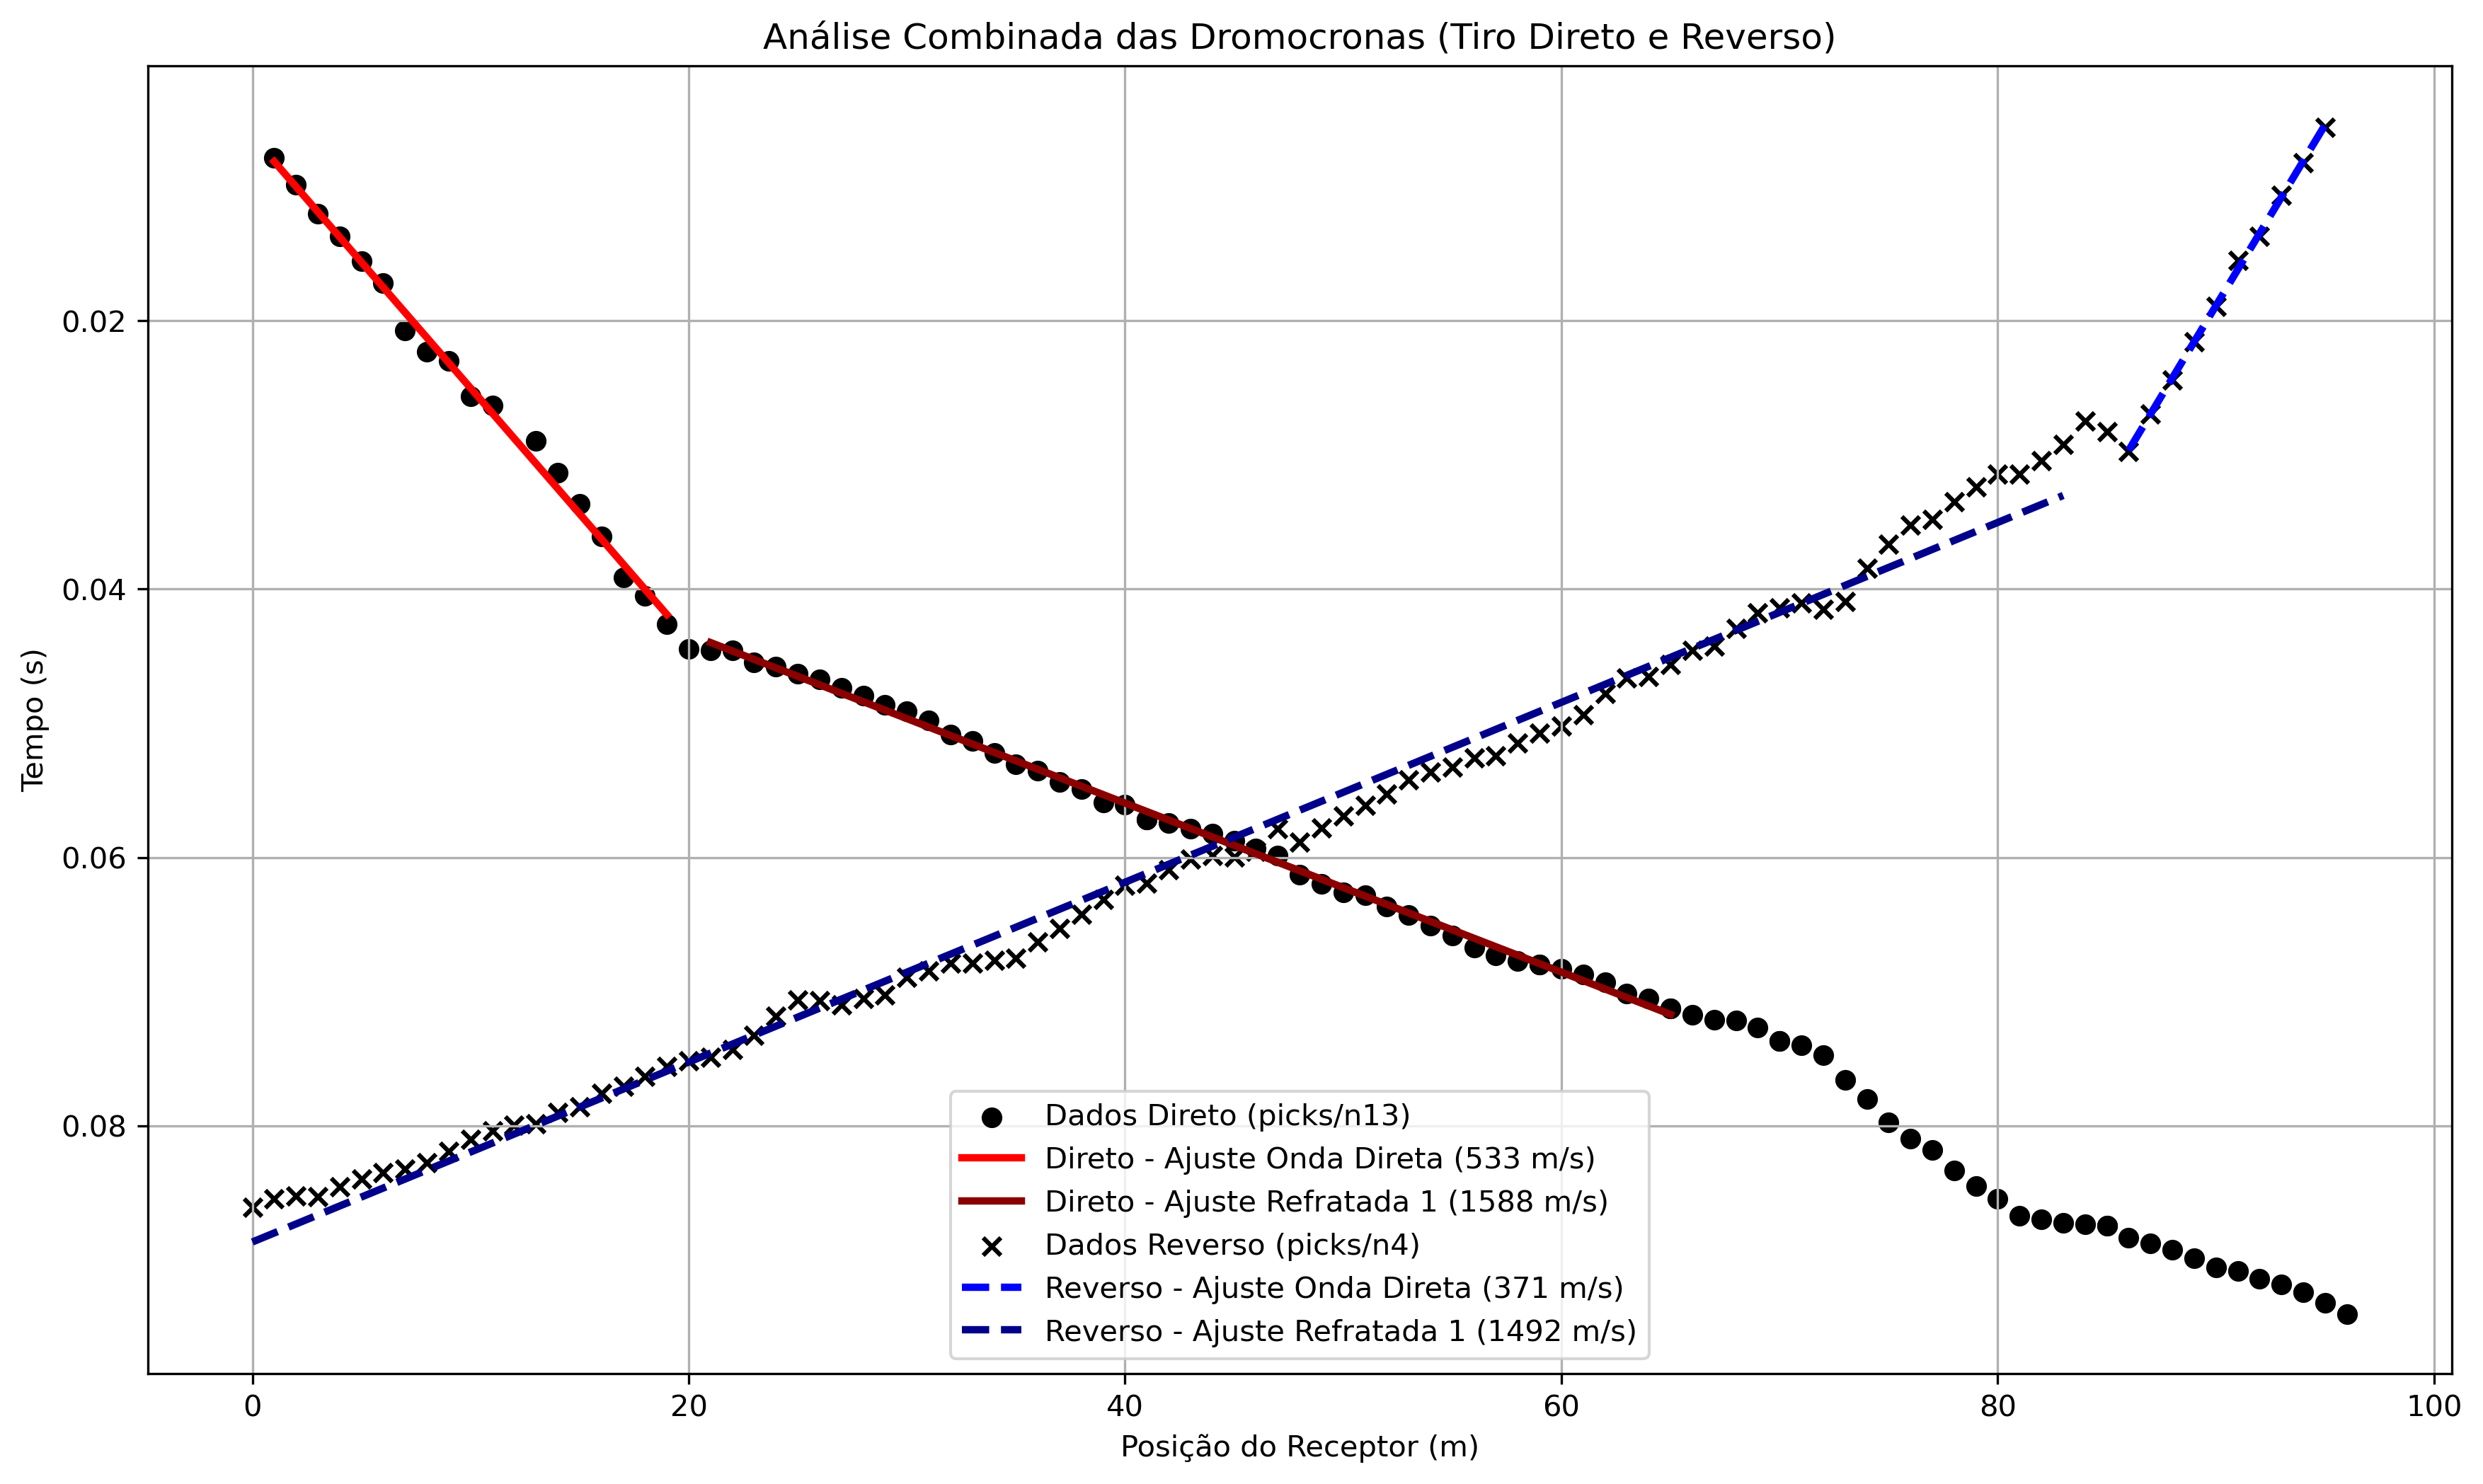
\includegraphics[width=0.5\linewidth]{dromocronas_combinadas.png}
    \caption{Análise combinada dos tiros 13 e 4.}
    \label{fig:placeholder}
\end{figure}


As figuras 10 e 11 mostram os resultados e estimativas obtidas a partir dos métodos e Interceptação e Recíproco, enquanto a figura 12 mostra os dois métodos plotados em um mesmo gráfico com menor nível de detalhamento em relação a profundidade abaixo de cada geofone.

\begin{figure}[H]
    \centering
    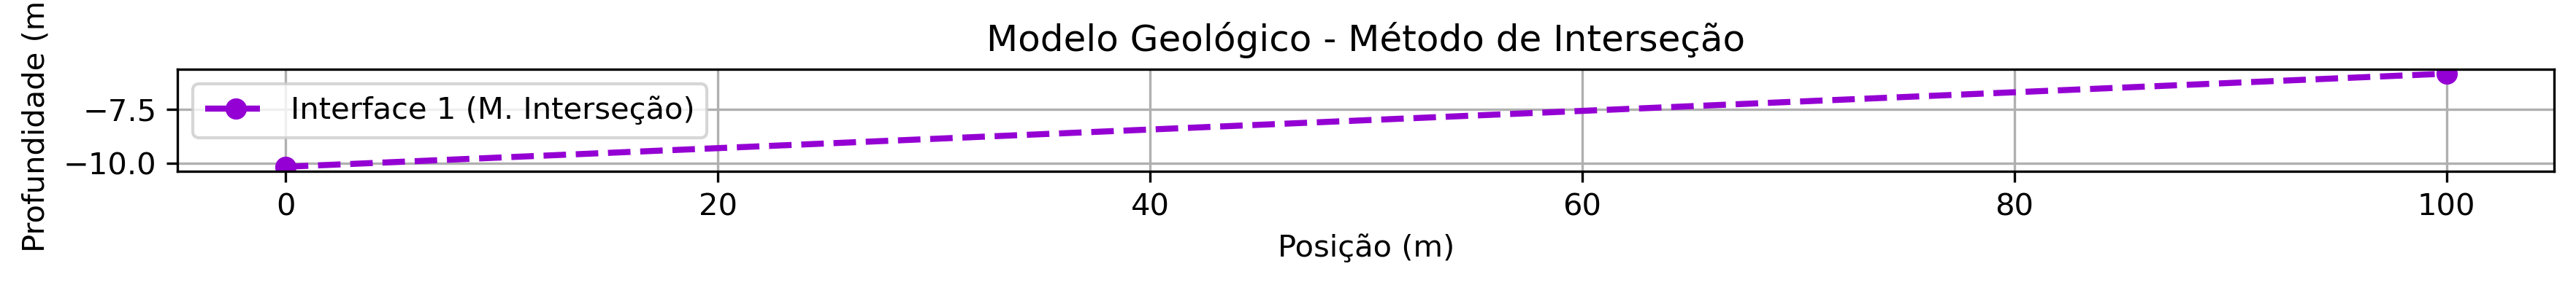
\includegraphics[width=0.5\linewidth]{interface_intersecao.png}
    \caption{Interface estimada a partir do método de interceptação.}
    \label{fig:placeholder}
\end{figure}

\begin{figure}[H]
    \centering
    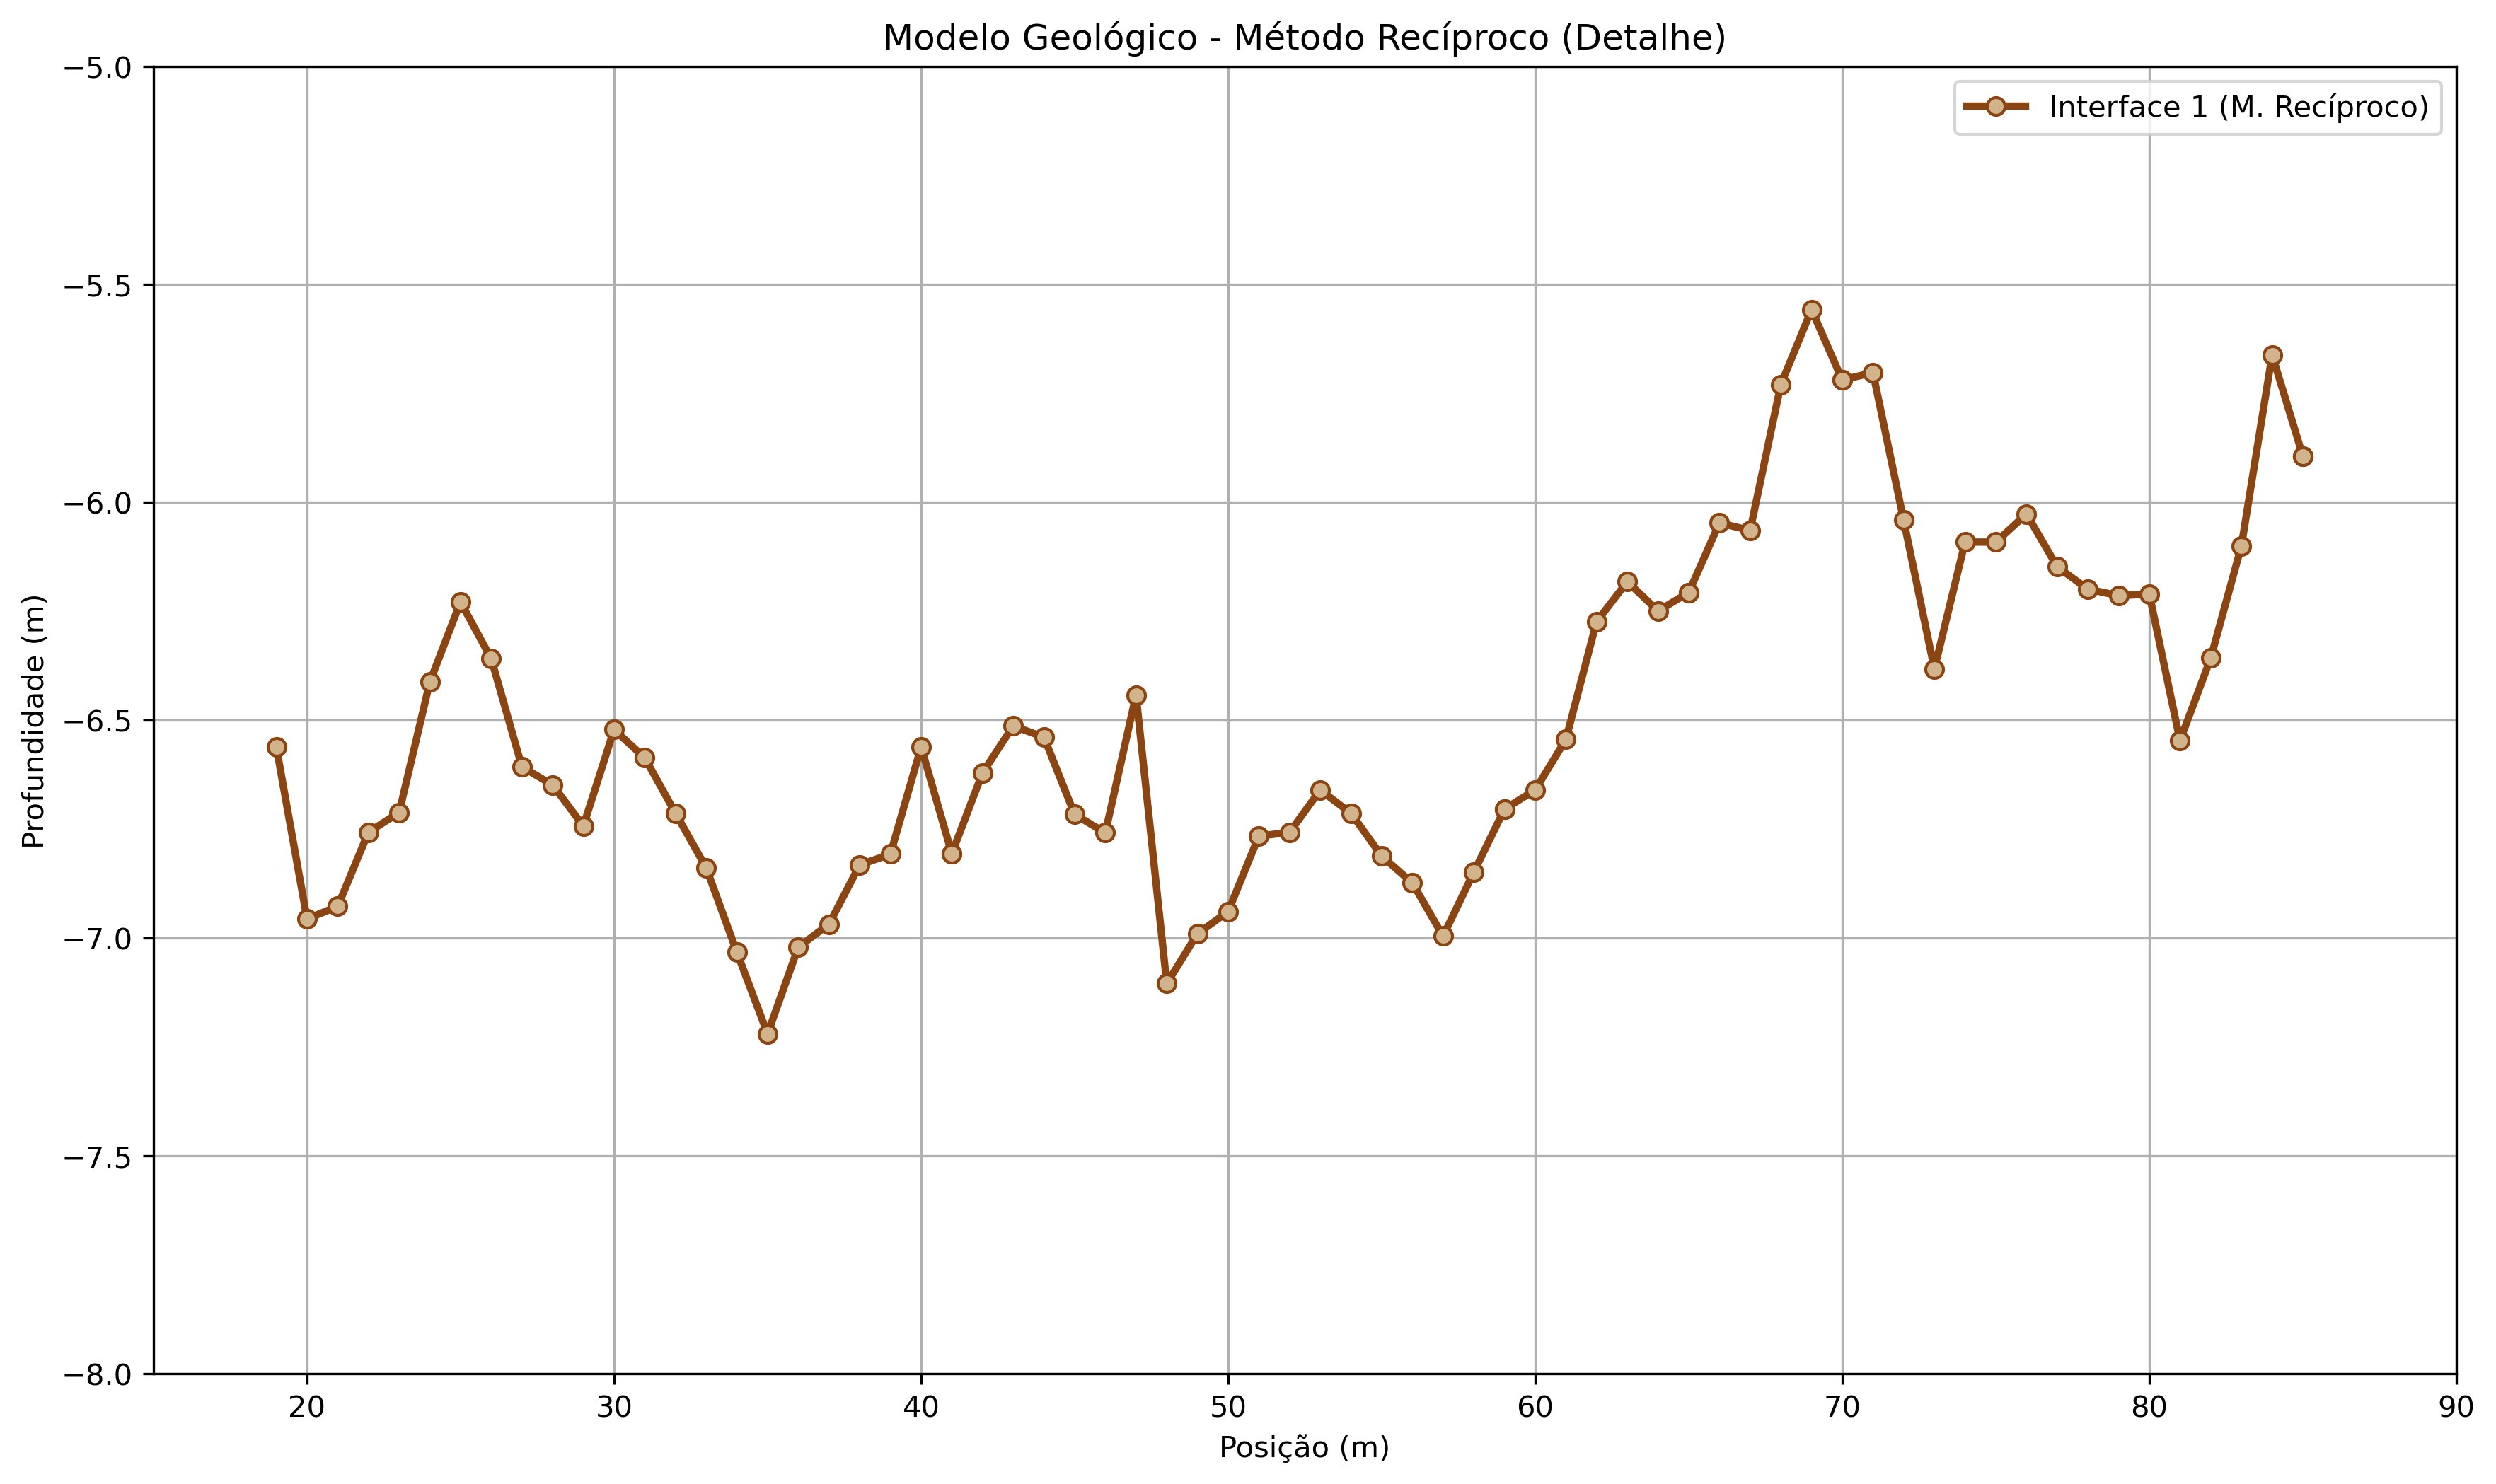
\includegraphics[width=0.5\linewidth]{interface_reciproco_detalhe.png}
    \caption{Interface estimada a partir do método recíproco, com maior detalhamento nas variações verticais de profundidade nos geofones.}
    \label{fig:placeholder}
\end{figure}


\begin{figure}[H]
    \centering
    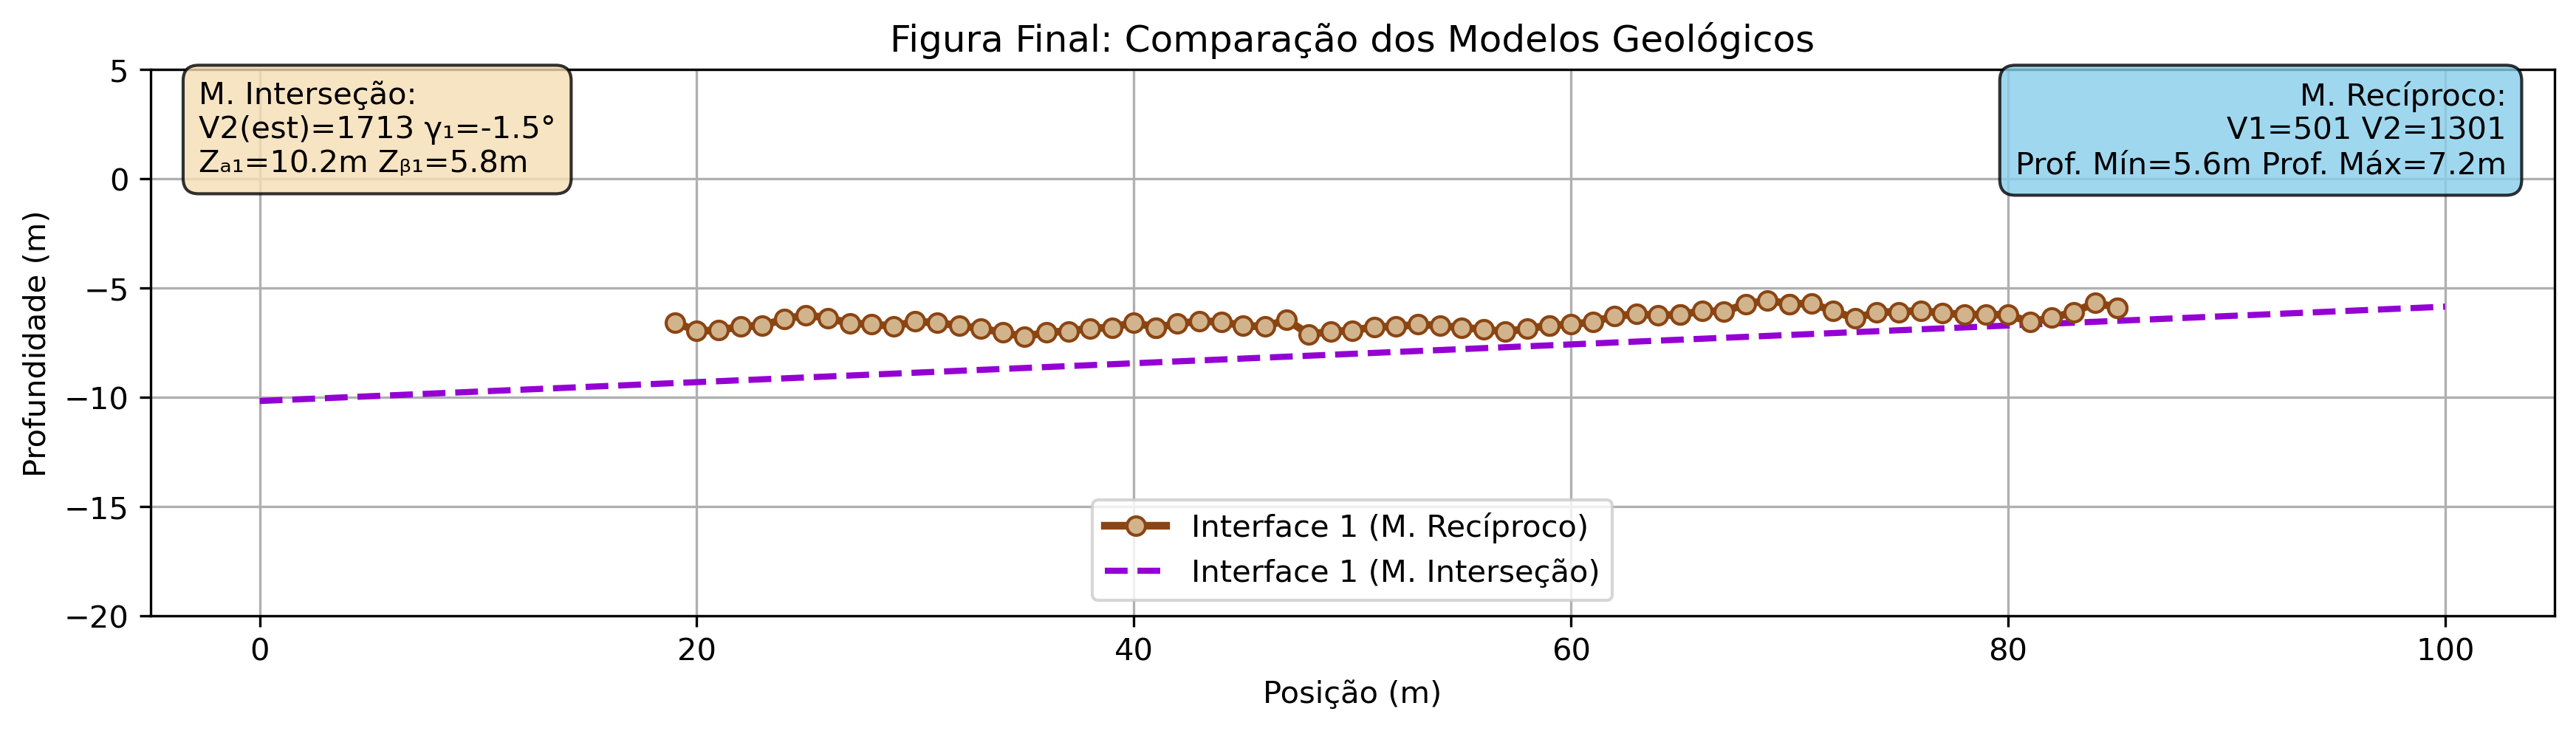
\includegraphics[width=0.5\linewidth]{interfaces_finais_comparativo.png}
    \caption{Comparação dos métodos, sem detalhamento na visualização.}
    \label{fig:placeholder}
\end{figure}


Utilizando os valores obtidos pelo método recíproco, presentes na legenda da figura 12, temos para a segunda camada velocidades de $V_{Direta} = 501m/s$ e $V_{refratada} = 1301 m/s$. A partir de uma consulta tabular, é possível ver os materiais compatíveis com esses valores de velocidade obtidos. Essa tabela está representada na figura 13.

\begin{figure}[H]
    \centering
    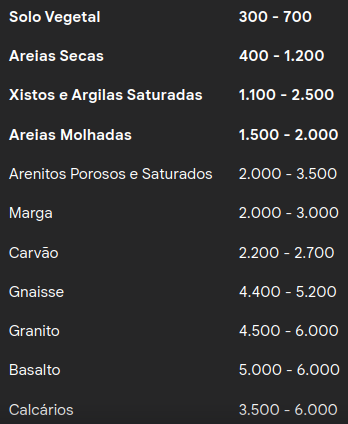
\includegraphics[width=0.5\linewidth]{tabela-velocidades0.png}
    \caption{Tabela com velocidades da onda p em diferentes meios (Fonte: GeoSci.xyz).}
    \label{fig:placeholder}
\end{figure}

A partir da tabela, a velocidade da onda direta foi compatível com solo vegetal e areias secas. Já a onda refratada foi compatível com xistos misturados à argila saturada e areias molhadas. Seria necessário um levantamento geológico mais preciso para maior credibilidade, mas com base na geologia local é possível inferir que de fato, a primeira camada era de solo vegetal. Para a segunda camada, não é possível afirmar sem um levantamengo e dados geológicos mais precisos. 




\section{Conclusão}

Os dados da Travessa C eram ruidosos, por conta principalmente da região de coleta e por serem mais antigos. Apesar disso, foi possível estimar a geometria da interface e fazer uma análise geológica plausível, com base nos parâmetros obtidos a partir da análise dos picks, e foi inferido que o modelo tinha apenas duas camadas e uma interface. A partir da tabela da figura 13 foi analisado quais meios são compatíveis com os resultados obtidos a fim de inferir a geologia local. A aplicação do método de sísmica de refração com suas ferramentas matemáticas para estimar velocidades e geometrias se mostrou, a princípio, eficaz para fazer uma análise do local de coleta de dados. 


\section{Prática 2025}

A disciplina teve uma prática com coleta de dados no ano de lançamento desse relatório. Essa prática foi pròxima ao ICB (Instituto de Ciencias Biológicas, figura 2) em uma região com relevante presença de ruídos, assim como a Travessa C. A montagem foi semelhante à descrita em Procedimentos, com as mesmas dificuldades explicadas. No entanto, não trabalhamos a fundo com os dados obtidos nessa prática, mas foi essencial para saber a dinâmica de trabalho em um campo. 



\end{document}